\documentclass[iop,twocolappendix]{emulateapj}
\usepackage{blindtext}
%\usepackage{float}
\usepackage{placeins}
\usepackage{graphicx}
\usepackage{amssymb, amsmath}
\usepackage{natbib}
\usepackage{amsmath}
\usepackage{bm}
\usepackage{color}
\usepackage[colorlinks,urlcolor=blue,citecolor=blue,linkcolor=blue]{hyperref}
%\usepackage{subfigure}
%\usepackage{caption}
%\usepackage{subcaption}
\interfootnotelinepenalty=10000
\usepackage[caption=false]{subfig}
\DeclareMathOperator{\sech}{sech}
\begin{document}
\title{Secondary Tearing Mode in trans-relativistic magnetic reconnection: dependence on plasma parameters}

\author{David Ball,\altaffilmark{1,3} Lorenzo Sironi,\altaffilmark{2} and Feryal \"Ozel\altaffilmark{1}}

\altaffiltext{1}{Department of Astronomy and Steward Observatory, Univ. of Arizona, 933 N. Cherry Avenue, Tucson, AZ 85721, USA}

\altaffiltext{2}{Department of Astronomy, Columbia University, 550 West 120th Street, New York, NY 10027, USA}
\altaffiltext{3}{Email: davidrball@email.arizona.edu}


\begin{abstract}
	We investigate how the onset of the secondary tearing mode depends on the intial plasma-$\beta$, magnetization $\sigma$, and strength of the guide field.  We explore how these physical parameters affect the structure and dynamics of the current layer, including the inflow and outflow velocities, outflow thickness
\end{abstract}

\keywords{magnetic reconnection --- accretion, accretion disks ---galaxies: jets ---X-rays: binaries --- radiation mechanisms: nonthermal --- acceleration of particles} 
\maketitle


\section{Introduction}
We showed in a previous paper that when the secondary tearing mode is active in a current sheet, that electron acceleration can occour along the entire length of the current sheet rather than only at primary x-points in the current sheet.  In this way, the secondary tearing mode will enable electron acceleration in large systems with thick current sheets, as expected astrophysically, where primary x-points will likely be limited.  As such, understading how the onset of the secondary tearing mode scales with various plasma parameters is crucial to understanding the resulting electron spectra from reconnection in astrophysical environments.  


\section{Methods}
We employ a large suite of PIC simulations with varying $\sigma$, $\beta$, and guide field strength expressed as a fraction of the strength of the initial in-plane component of the magnetic field, $R_{g}=B_{g}/B_{0}$.  


\section{Inflow and Outflow Rates}

\begin{figure}[!h]
	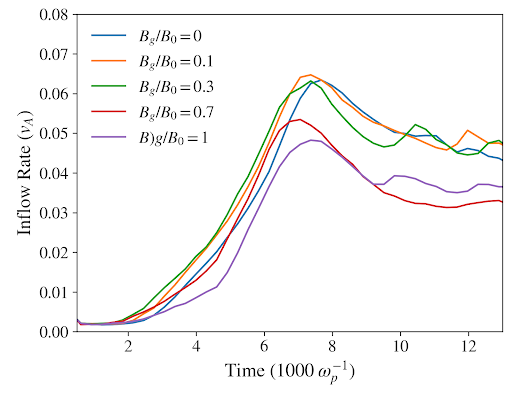
\includegraphics[width=\linewidth]{sig_3_highbeta_inflows.png}
	\caption{Inflow rate from a set of simulations with $\sigma=0.3 \; \beta=0.3$ and varying guide field strengths.  We see that for low guide field strengths $\leq 0.3$, that the inflow rates are roughly comparable.  As the guide field strengths increase beyond this, however, the inflow rates sbegin to decrease.
	}
	\label{sig.3_highbeta_inflows}
\end{figure}

\begin{figure}[!h]
	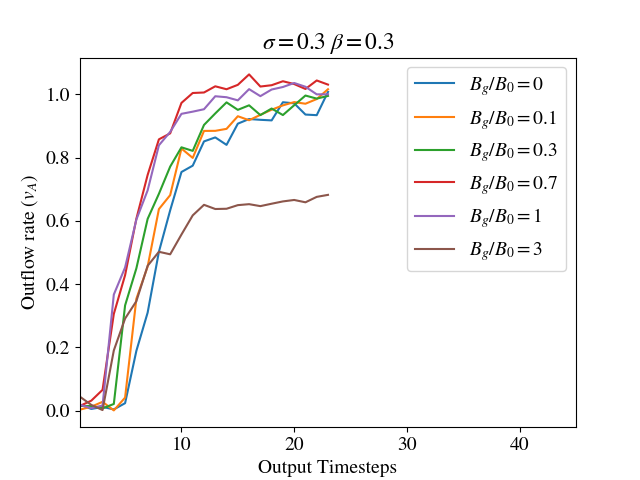
\includegraphics[width=\linewidth]{sig_3_highbeta_outflows_sweetspot.png}
	\caption{Outflow rate from a set of simulations with $\sigma=0.3 \; \beta=0.3$ and varying guide field strengths.  We see that when the guide field strength is low, that the outflow speeds tend to increase with increasing guide field strength.  This is because the increased guide fields begin to suppress the firehose instability, which slows down the outflows.  Once the firehose instability is completely suppressed (around  $B_{g}=0.7B_{0}$), the increasing guide field lowers the outflow speed due to the increase in relativistic energy density contained in the outflow.
	}
	\label{sig.3_highbeta_outflows}
\end{figure}


\begin{figure}[!h]
	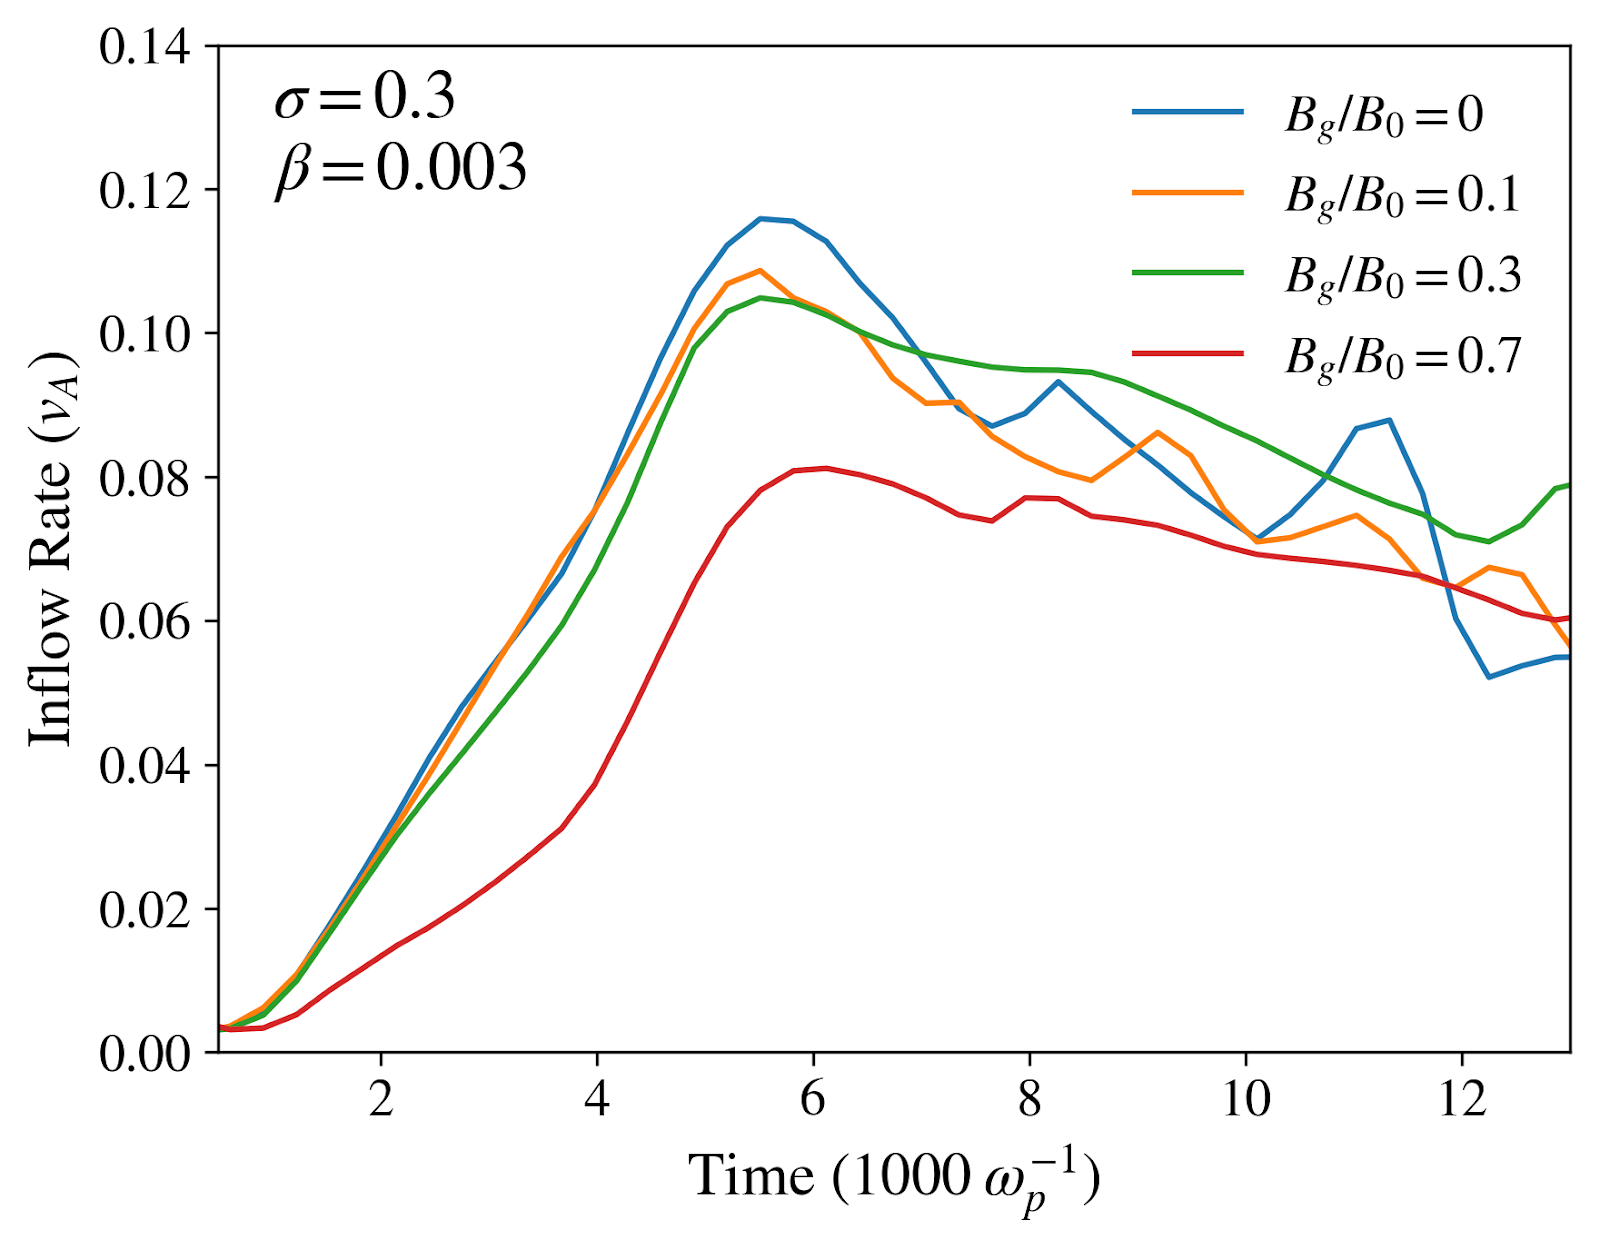
\includegraphics[width=\linewidth]{sig_3_lowbeta_inflows.png}
	\caption{Inflow rate from a set of simulations with $\sigma=0.3 \; \beta=0.003$ and varying guide field strengths.  We see in this low-$\beta$ case that as the guide field strength increases, it slows down the inflow velocity due to the additional inertia of the mildly relativistic guide fields.
	}
	\label{sig.3_lowbeta_inflows}
\end{figure}

\begin{figure}[!h]
	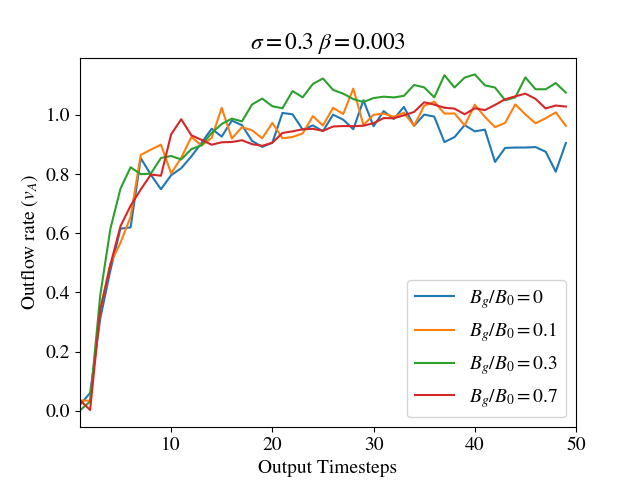
\includegraphics[width=\linewidth]{sig_3_lowbeta_outflows.png}
	\caption{Outflow rate from a set of simulations with $\sigma=0.3 \; \beta=0.003$ and varying guide field strengths. 
	}
	\label{sig.3_lowbeta_outflows}
\end{figure}



\section{Current Sheet Width}
\begin{figure}[!h]
	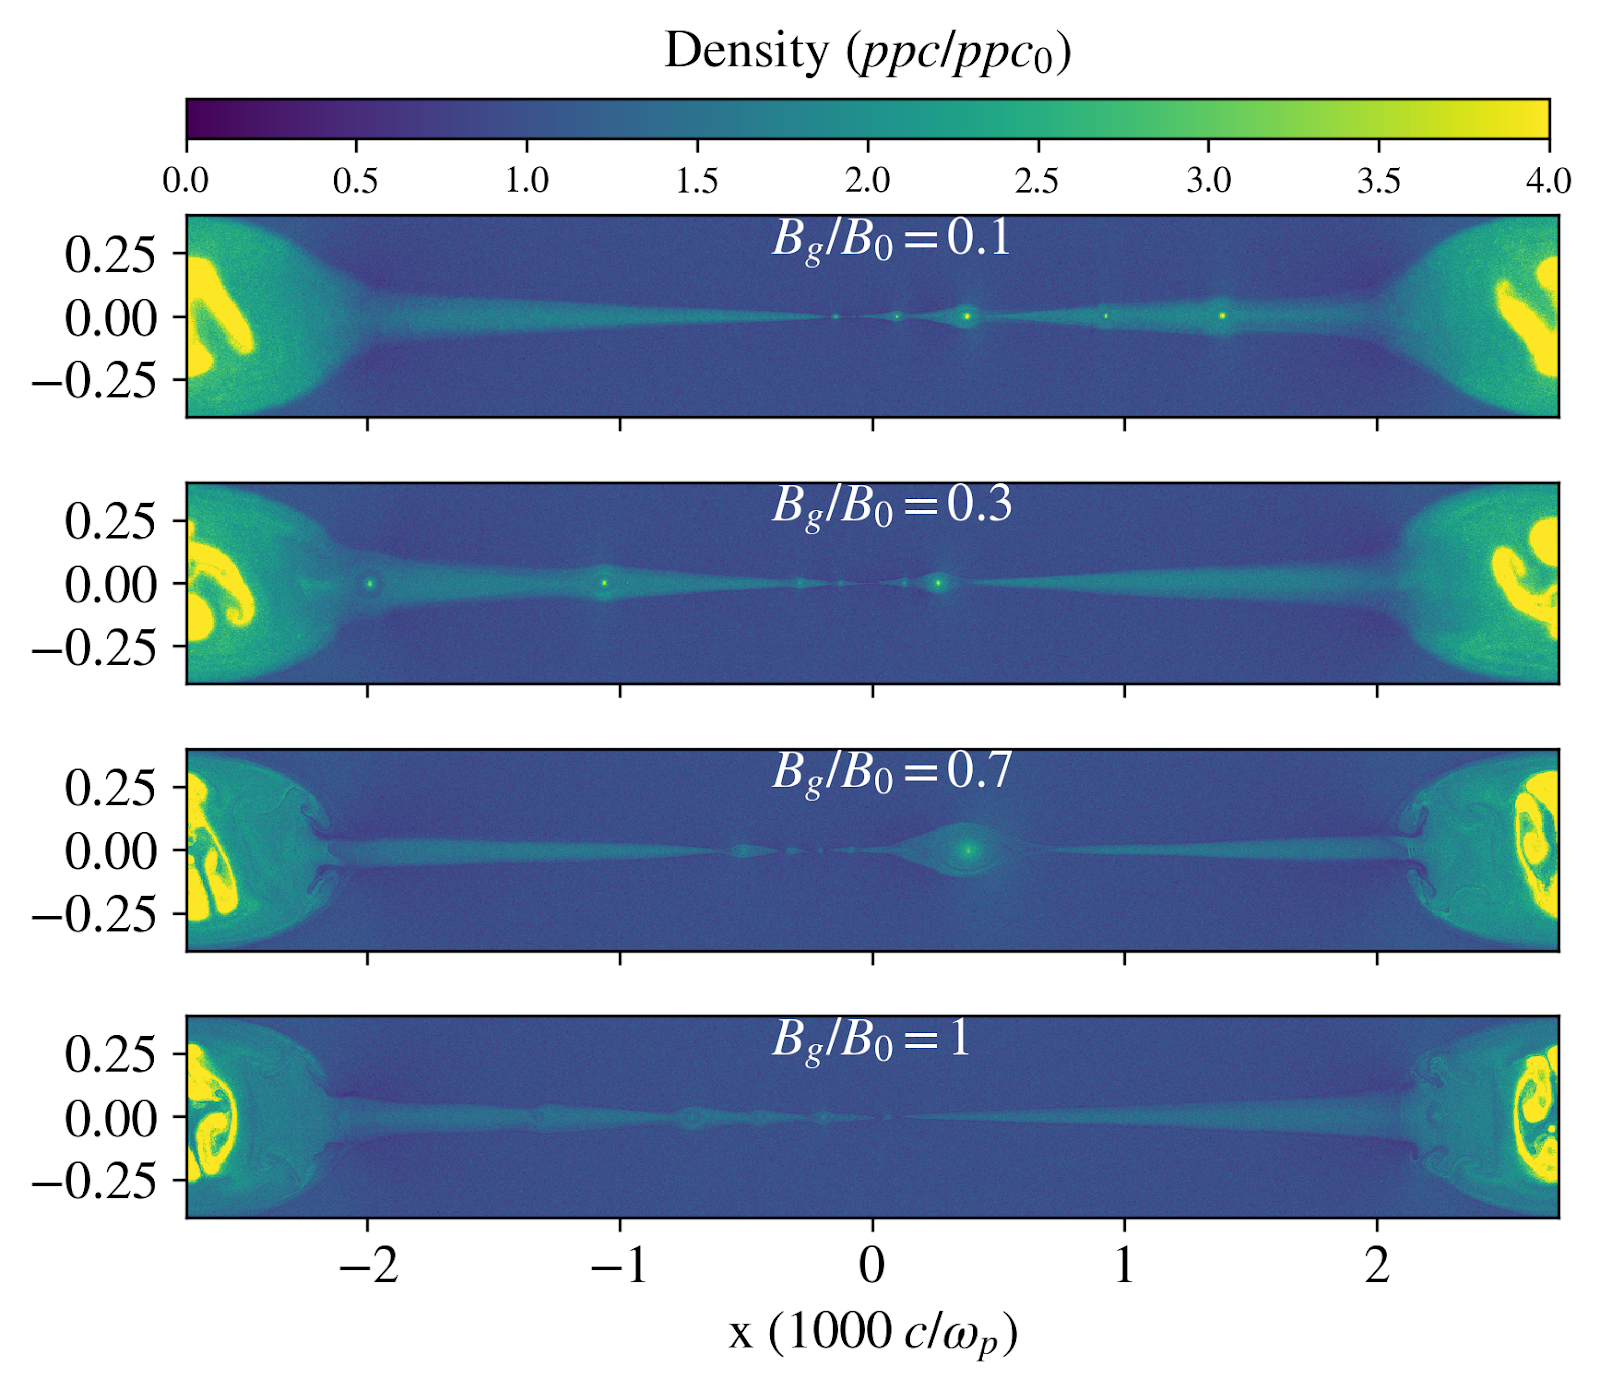
\includegraphics[width=\linewidth]{sig_3_highbeta_outflow_flds.png}
	\caption{Density profiles for the set of simulations with $\sigma=0.3 \; \beta=0.3$ at varying guide field strengths.  By eye, we can see that the width of the current layer decreases from $B_{g}=0.1 B_{0}$ to $B{g}=0.7B_{0}$, and then increases as the guide field increases beyond this.
	}
	\label{highbeta_outflow_flds}
\end{figure}

\begin{figure}[!h]
	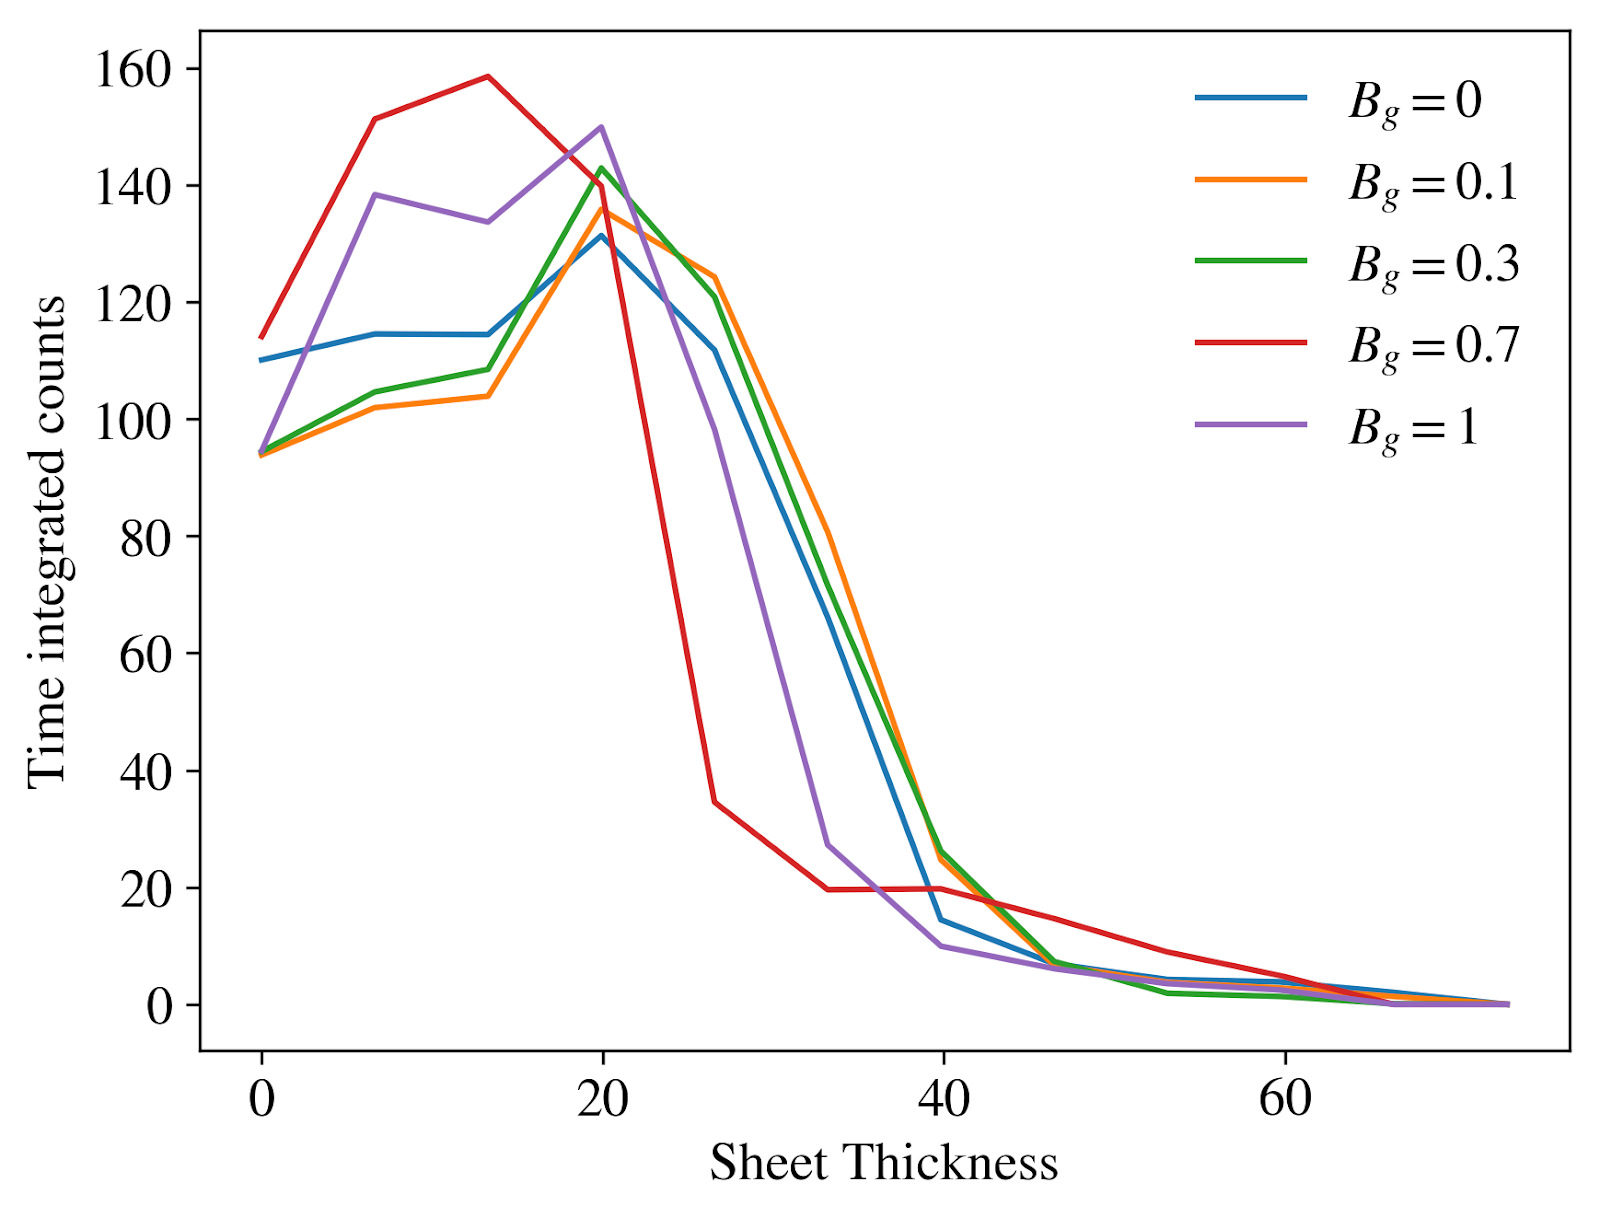
\includegraphics[width=\linewidth]{sig_3_highbeta_thickness.png}
	\caption{Histograms of current sheet thicknesses for the four simulations shown above in Figure \ref{highbeta_outflow_flds} as well as an additional case with $B_{g}=0$.  We see that when the guide field is small, the current sheet has typical widths of $\sim30$.  At a guide field stregnth of $0.7$, the magnetic field strength is strong enough to control the firehose instability and the outflows speed up, resulting in thinner sheets.  As the guide field strenght increases beyond this, however, the outflows slow down again due to the relativistic energy density of the stronger guide fields, and the current sheets again begin to thicken.}
	
	\label{highbeta_outflow_thickness}
\end{figure}




\section{Average Density in Current Sheet}
\begin{figure}[!h]
	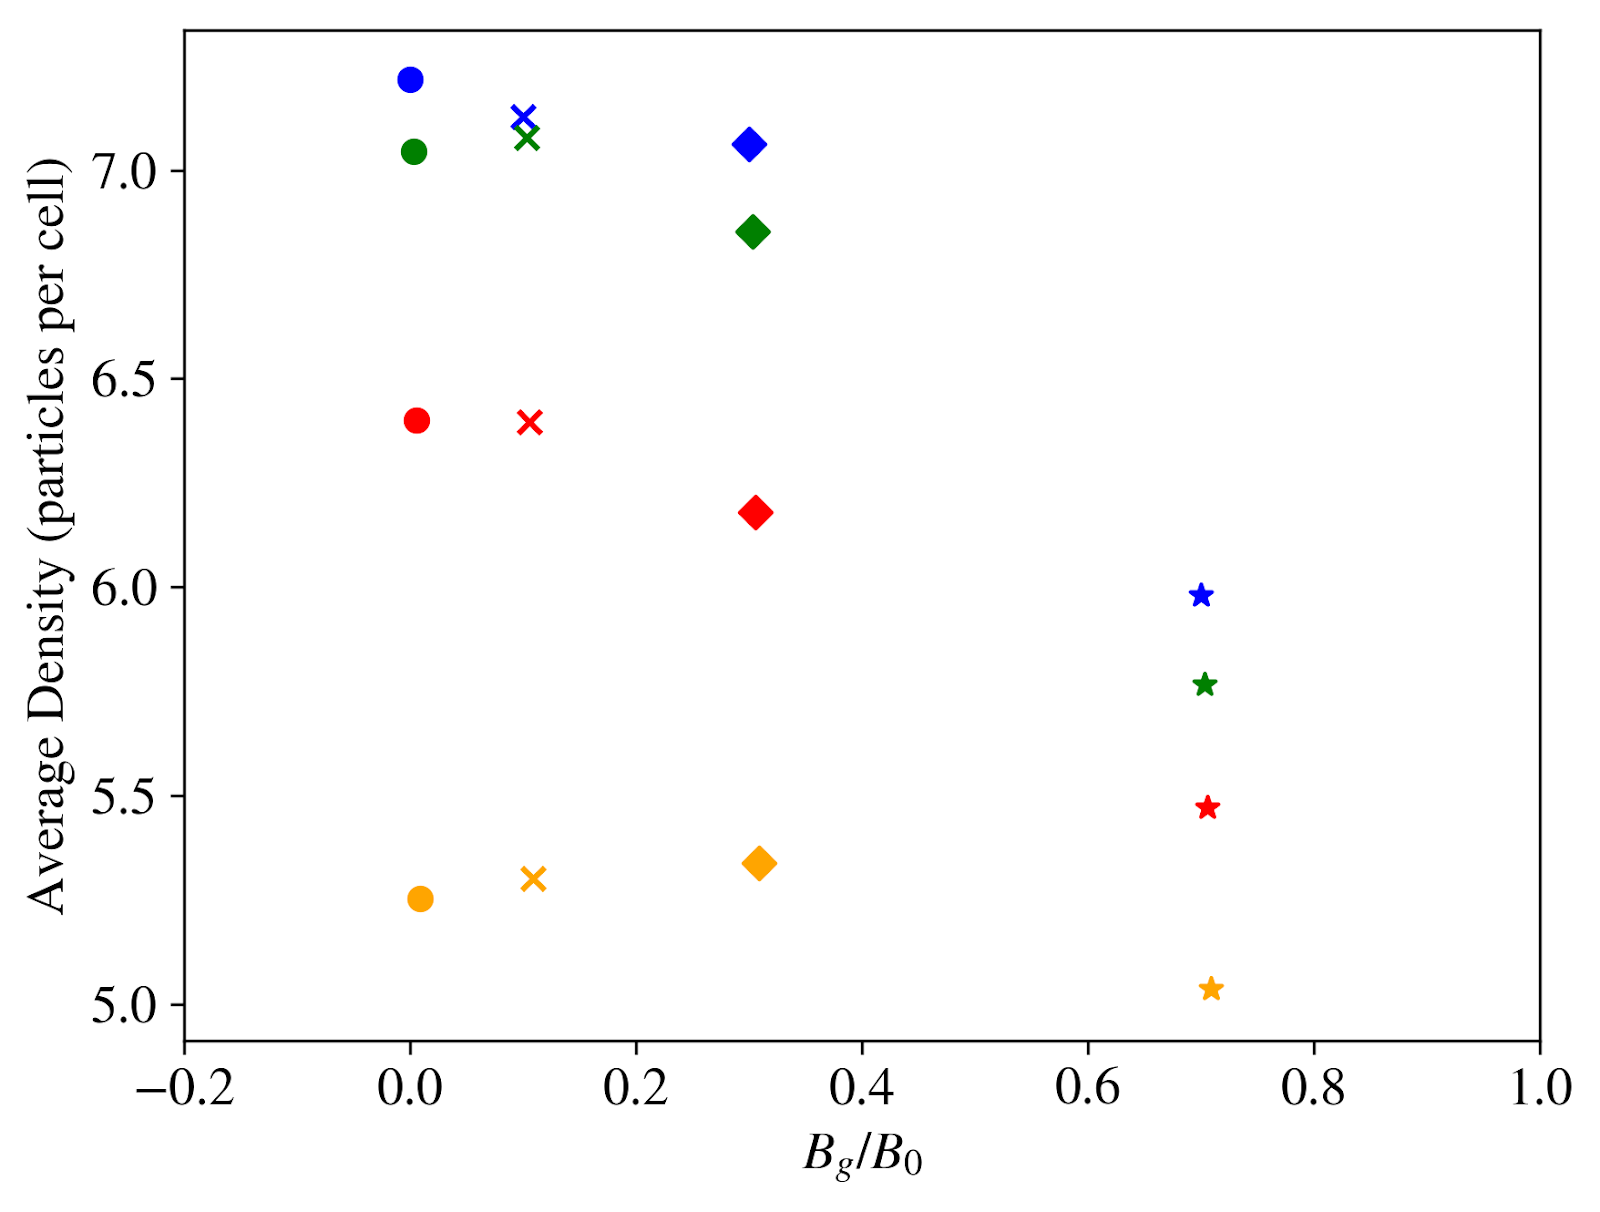
\includegraphics[width=\linewidth]{sig_3_bguide_vs_dens.png}
	\caption{Guide field strength vs. average density in the outflows for our set of $\sigma=0.3$ simulations.  The color corresponds to the plasma $\beta$, with blue, green, red, and orange, corresponding to $\beta=0.0003, \; 0.003,  \; 0.03, \;0.3 $, respectively.  We see at low-$\beta$ that the average density in the outflows depend quite sensetively on the guide field, whereas at higher-$\beta$, increasing the guide field has much less drastic effect.  This is because at high-$\beta$, the current sheet is already supported by the thermal pressure of the plasma, so changing the strength of the guide field does not have much of an effect on the overall dynamics of the current layer.  However when the thermal pressure is small, the guide field stabalizes the current sheet, increasing its width and thereby stabalizing it against the secondary tearing instability, and results in thicker, less dens outflows.
	}
	\label{highbeta_outflow_flds}
\end{figure}


\section{Interpretations via the Equation of Continuity}
Tie together results from the previous three sections where the inflow/outflow rates, current sheet widths, and average density in the sheet via the equation of continuity, can it explain our results?


\section{Secondary tearing and the formation of x-points and plasmoids}
How do all the above pieces fit together to form a pictures of when the secondary tearing mode is active.



\section{Appendix A: Density snapshots across parameter scans}


\begin{figure*}[!h]
	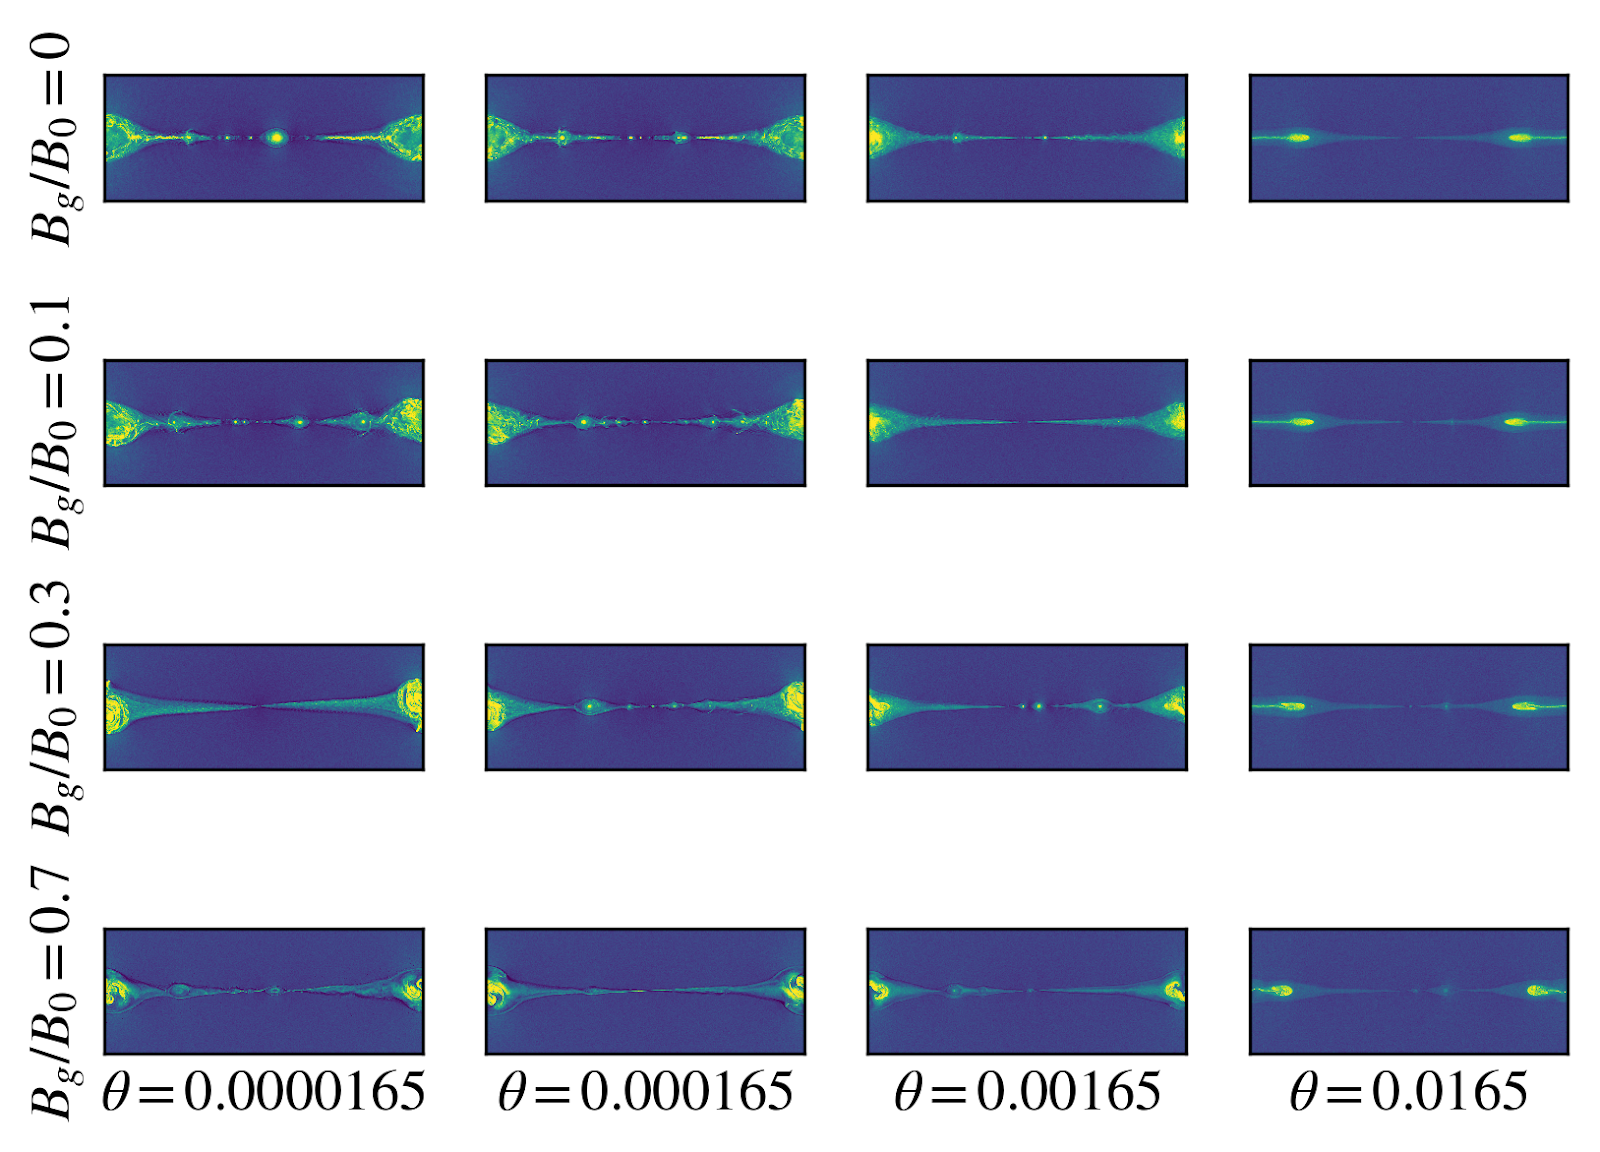
\includegraphics[width=\linewidth]{sig_1_params.png}
	\caption{Density structures for our $\sigma=0.1$ simulations across $\theta$ and $B_{g}/B_{0}$.
	}
	\label{sig.1_matrix}
\end{figure*}

\begin{figure*}[!h]
	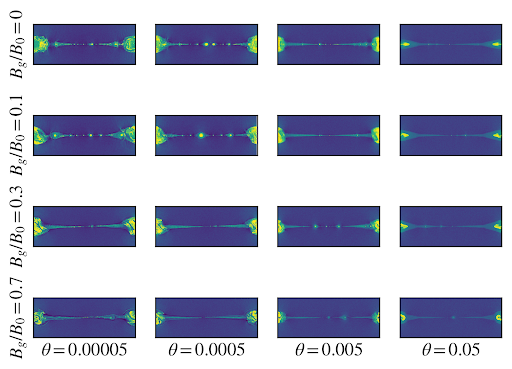
\includegraphics[width=\linewidth]{sig_3_params.png}
	\caption{Density structures for our $\sigma=0.3$ simulations across $\theta$ and $B_{g}/B_{0}$.
	}
	\label{sig.3_matrix}
\end{figure*}

\begin{figure*}[!h]
	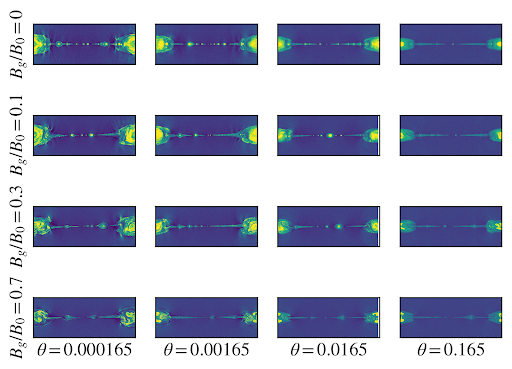
\includegraphics[width=\linewidth]{sig1_params.png}
	\caption{Density structures for our $\sigma=1$ simulatios across $\theta$ and $B_{g}/B_{0}$.
	}
	\label{sig1_matrix}
\end{figure*}





\end{document}